\section{Network Monitoring :}
\subsection{Live Network Monitoring:}
\subsubsection{Simulation :}


\begin{itemize}
    \item Determine the active network interfaces on the system by executing the ip a command. This step is essential for identifying the interface through which network traffic will be monitored.
\end{itemize}

\begin{figure}[H]
    \centering
    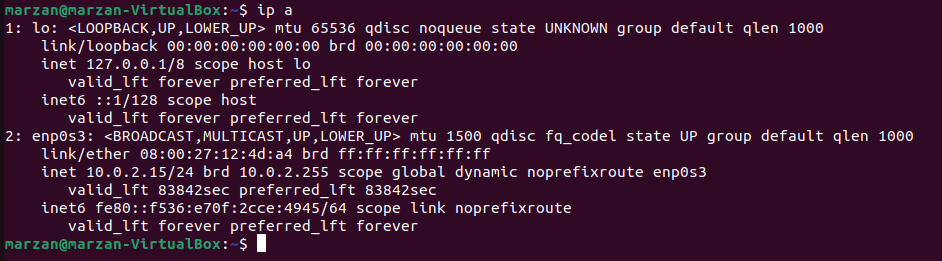
\includegraphics[width=1\linewidth]{images/ipa.png}
    \caption{live network interfaces}
    \label{fig:enter-label}
\end{figure}

\begin{itemize}
    \item Configure the Zeek node by editing the node.cfg file. Specify the network interface to be monitored by adding the line interface=enp0s3.
\end{itemize}


\begin{figure}[H]
    \centering
    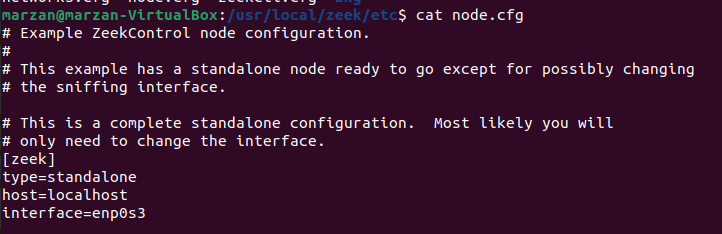
\includegraphics[width=1\linewidth]{images//live_monitor/node.png}
    \caption{node.cfg update}
    \label{fig:enter-label}
\end{figure}

\begin{itemize}
    \item Utilize the zeekctl command-line utility to manage the Zeek instance. Initiate Zeek by executing zeekctl start, and when necessary, halt the monitoring process using zeekctl stop.
\end{itemize}


\begin{figure}[H]
    \centering
    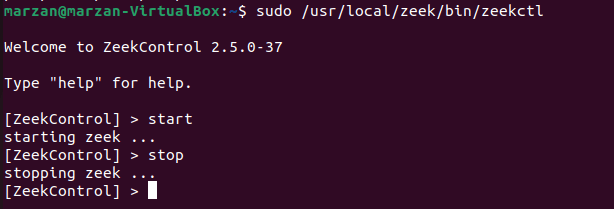
\includegraphics[width=1\linewidth]{images/live_monitor/zeekctl.png}
    \caption{zeekctl}
    \label{fig:enter-label}
\end{figure}

\begin{itemize}
    \item To ascertain the installation path of the zeekctl utility, employ the command which zeekctl. This command reveals the full path to the zeekctl executable, facilitating its execution.
\end{itemize}


\begin{figure}[H]
    \centering
    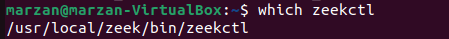
\includegraphics[width=1\linewidth]{images/live_monitor/which zeekctl.png}
    \caption{zeekctl path}
    \label{fig:enter-label}
\end{figure}

\begin{itemize}
    \item Activate the Zeek control application by executing start zeekctl, which initiates the live monitoring process.
\end{itemize}

\begin{figure}[H]
    \centering
    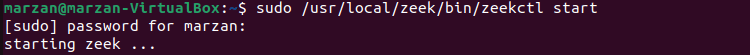
\includegraphics[width=1\linewidth]{images/live_monitor/zeetctl_start.png}
    \caption{zeekctl start}
    \label{fig:enter-label}
\end{figure}
\begin{itemize}
    \item Upon commencement of live monitoring, Zeek begins to capture and analyze network traffic, systematically storing the results in a series of log files. These logs, encompassing various protocols and activities, include but are not limited to dns.log, http.log, and dhcp.log.
\end{itemize}

\begin{figure}[H]
    \centering
    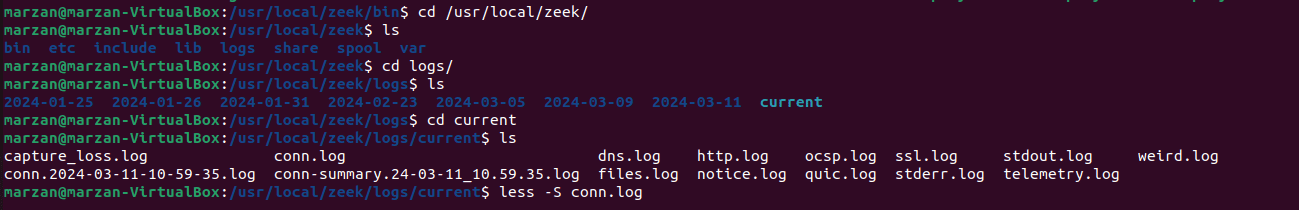
\includegraphics[width=1\linewidth]{images/live_monitor/live_logs.png}
    \caption{Log files}
    \label{fig:enter-label}
\end{figure}

\begin{itemize}
    \item To examine the connection log (conn.log), the command less -S conn.log is employed. This command provides a paginated view of the conn.log file, allowing for detailed inspection of recorded network connections.
\end{itemize}


\begin{figure}[H]
    \centering
    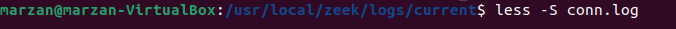
\includegraphics[width=1\linewidth]{images/live_monitor/less_conn_live.png}
    \caption{conn.log}
    \label{fig:enter-label}
\end{figure}

\begin{itemize}
    \item Further scrutiny of the conn.log file can be achieved through direct observation, facilitating a deeper understanding of the network interactions and anomalies.
\end{itemize}


\begin{figure}[H]
    \centering
    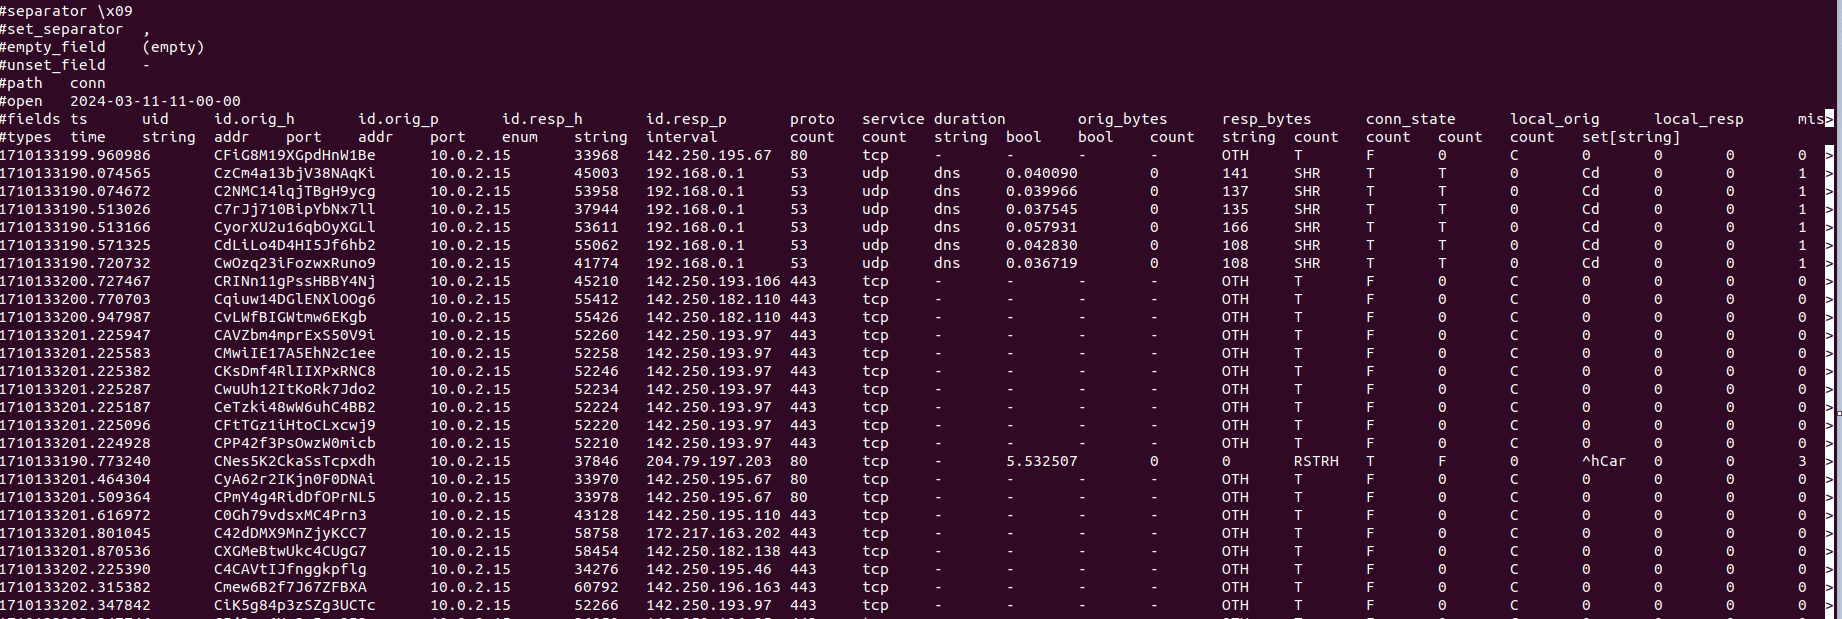
\includegraphics[width=1\linewidth]{images/new_1.png}
    \caption{conn.log}
    \label{fig:enter-label}
\end{figure}

\begin{itemize}
    \item For an enhanced analysis experience, the conn.log file may be imported into the Brim application. Brim provides a graphical interface for interacting with Zeek logs, offering advanced search capabilities and visualizations to aid in the interpretation of network data.
\end{itemize}

\begin{figure}[H]
    \centering
    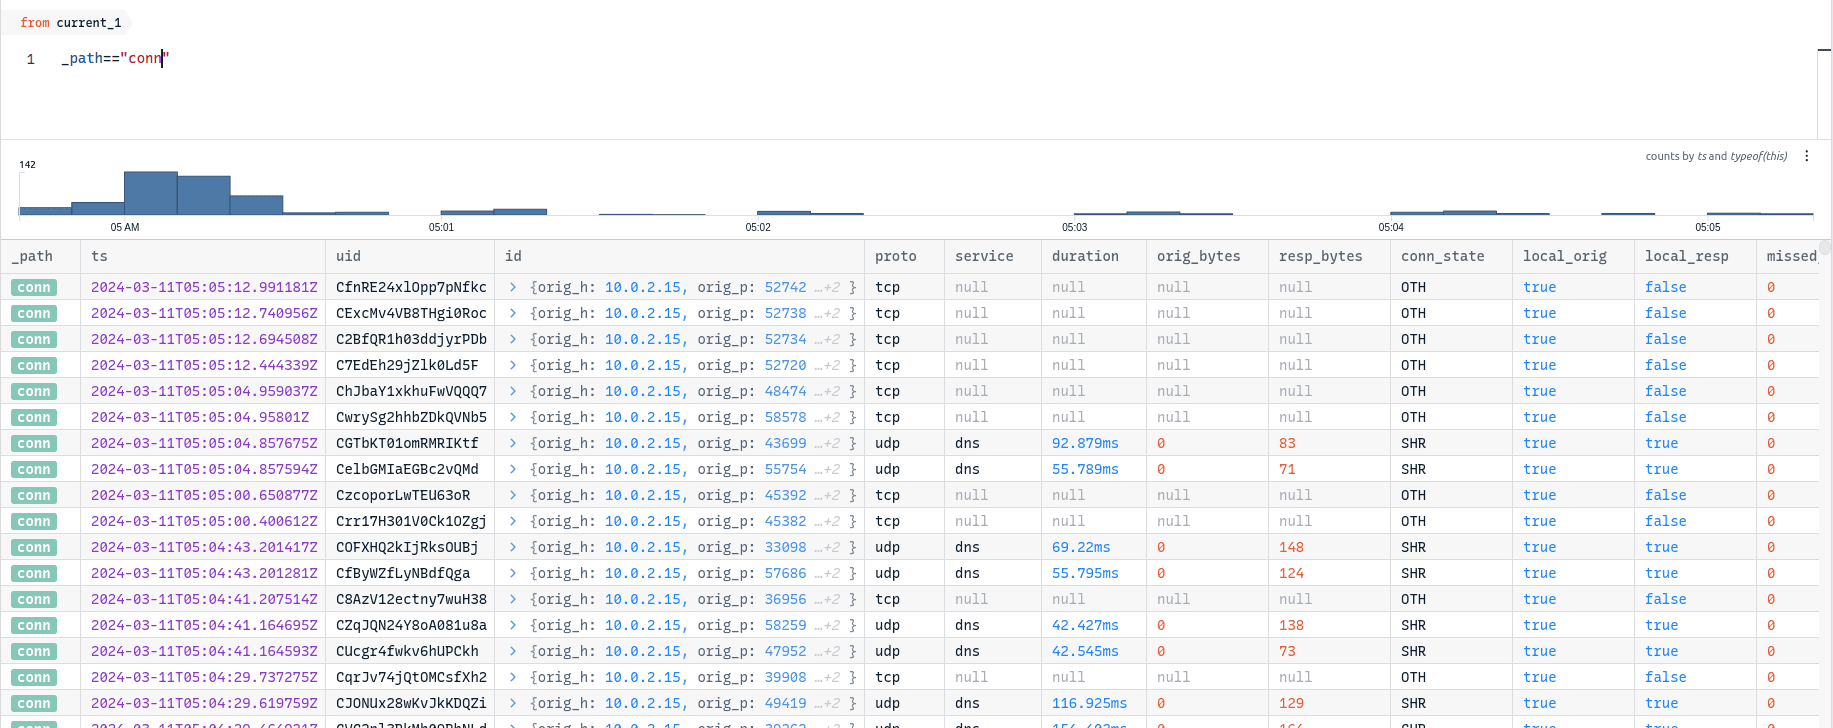
\includegraphics[width=1\linewidth]{images/live_monitor/live_brim_conn.png}
    \caption{conn.log in BRIM}
    \label{fig:enter-label}
\end{figure}

\begin{itemize}
    \item To check out the DNS activity,we have opened the dns.log file using less -S dns.log. This shows the DNS details page by page, making it easier to see what's happening.
\end{itemize}

\begin{figure}[H]
    \centering
    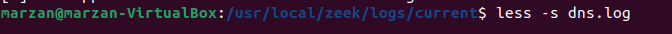
\includegraphics[width=1\linewidth]{images/live_monitor/less_dns_live.png}
    \caption{dns.log}
    \label{fig:enter-label}
\end{figure}

\begin{itemize}
    \item Direct analysis of dns.log elucidates DNS traffic patterns and anomalies.
\end{itemize}


\begin{figure}[H]
    \centering
    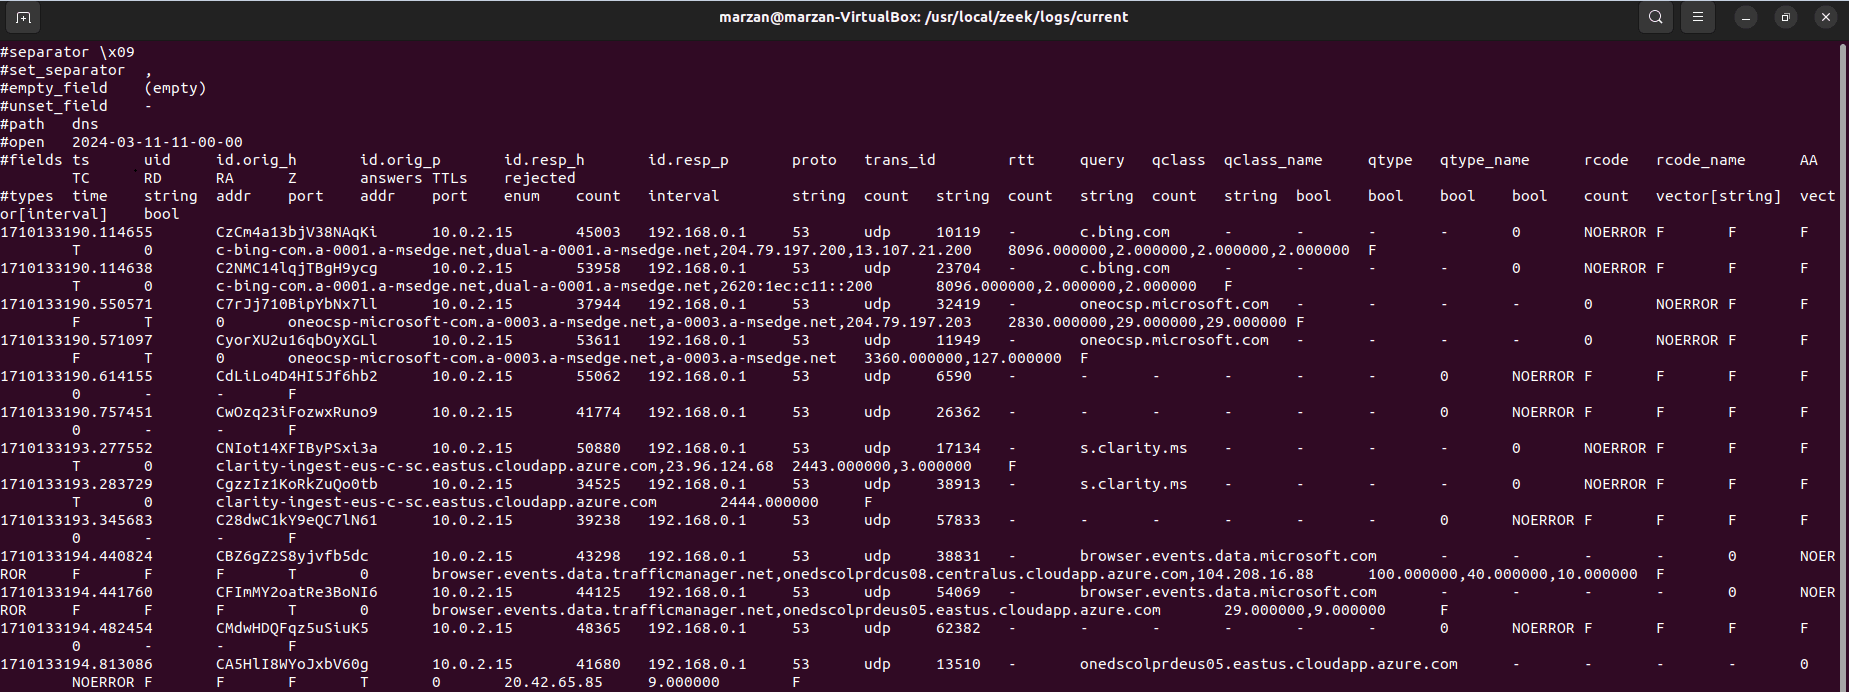
\includegraphics[width=1\linewidth]{images/new_2.png}
    \caption{dns.log}
    \label{fig:enter-label}
\end{figure}

\begin{itemize}
    \item For advanced analysis, dns.log is imported into Brim. Brim's GUI and analytical tools enhance DNS log data interpretation, offering clarity on network DNS behavior.
\end{itemize}

\begin{figure}[H]
    \centering
    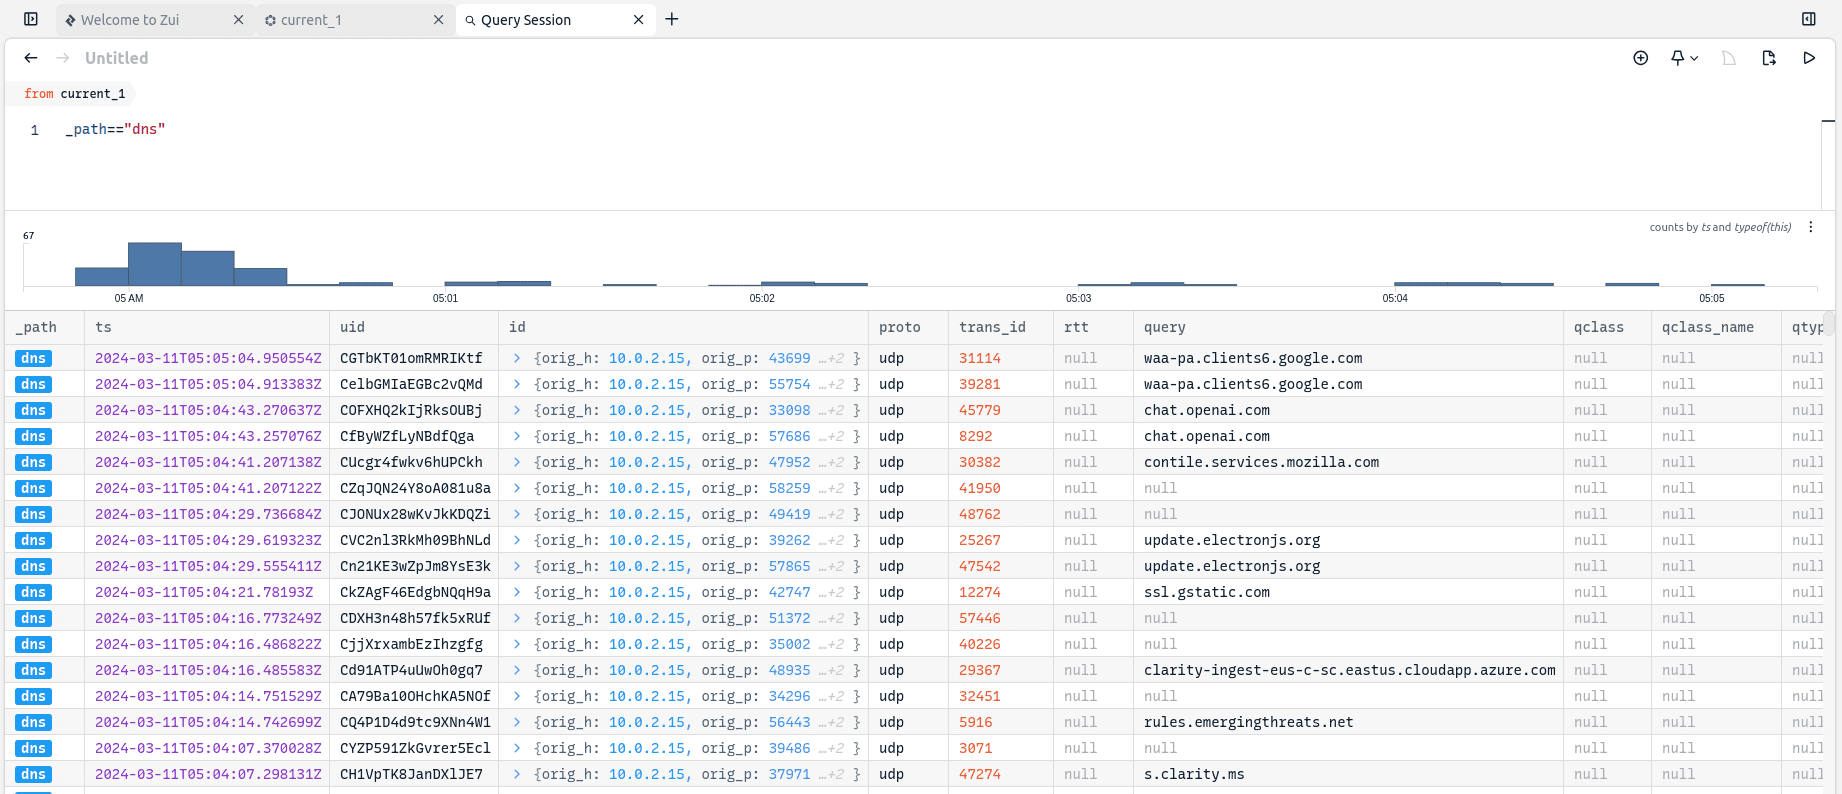
\includegraphics[width=1\linewidth]{images/live_monitor/live_brim_dns.png}
    \caption{dns.log in BRIM}
    \label{fig:enter-label}
\end{figure}



\subsection{Network Monitoring from PCAP file:}

Here is the link to PCAP file:
\href{https://www.malware-traffic-analysis.net/tutorials/index.html}{malware-traffic-analysis}\\\\

\subsubsection{Simulation :}
\begin{itemize}
    \item Begin by executing the command zeek -C -r a.pcap, which initiates the analysis of the provided PCAP file. The -C flag is used to ignore checksums, ensuring that all packets are analyzed irrespective of checksum validity.
\end{itemize}

\begin{figure}[H]
    \centering
    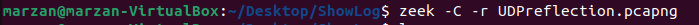
\includegraphics[width=1\linewidth]{images/pcap/pcap_1.png}
    \caption{zeek analysis of pcap file }
    \label{fig:enter-label}
\end{figure}

\begin{itemize}
    \item Upon completion of the analysis, Zeek will generate a series of log files, including but not limited to conn.log, dns.log, and weird.log, each containing detailed information pertinent to their respective network protocols and events.
\end{itemize}


\begin{figure}[H]
    \centering
    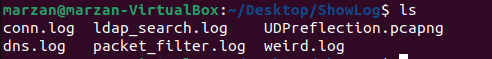
\includegraphics[width=1\linewidth]{images/pcap/pcap_2.png}
    \caption{Log files}
    \label{fig:enter-label}
\end{figure}

\begin{itemize}
    \item To review the DNS activity captured during the analysis, employ the command less -S dns.log. This command will present the contents of the dns.log file in a paginated manner, allowing for a detailed examination of DNS transactions.
\end{itemize}


\begin{figure}[H]
    \centering
    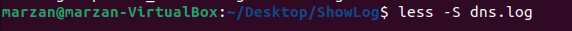
\includegraphics[width=1\linewidth]{images/pcap/pcap_4.png}
    \caption{dns.log}
    \label{fig:enter-label}
\end{figure}


\begin{figure}[H]
    \centering
    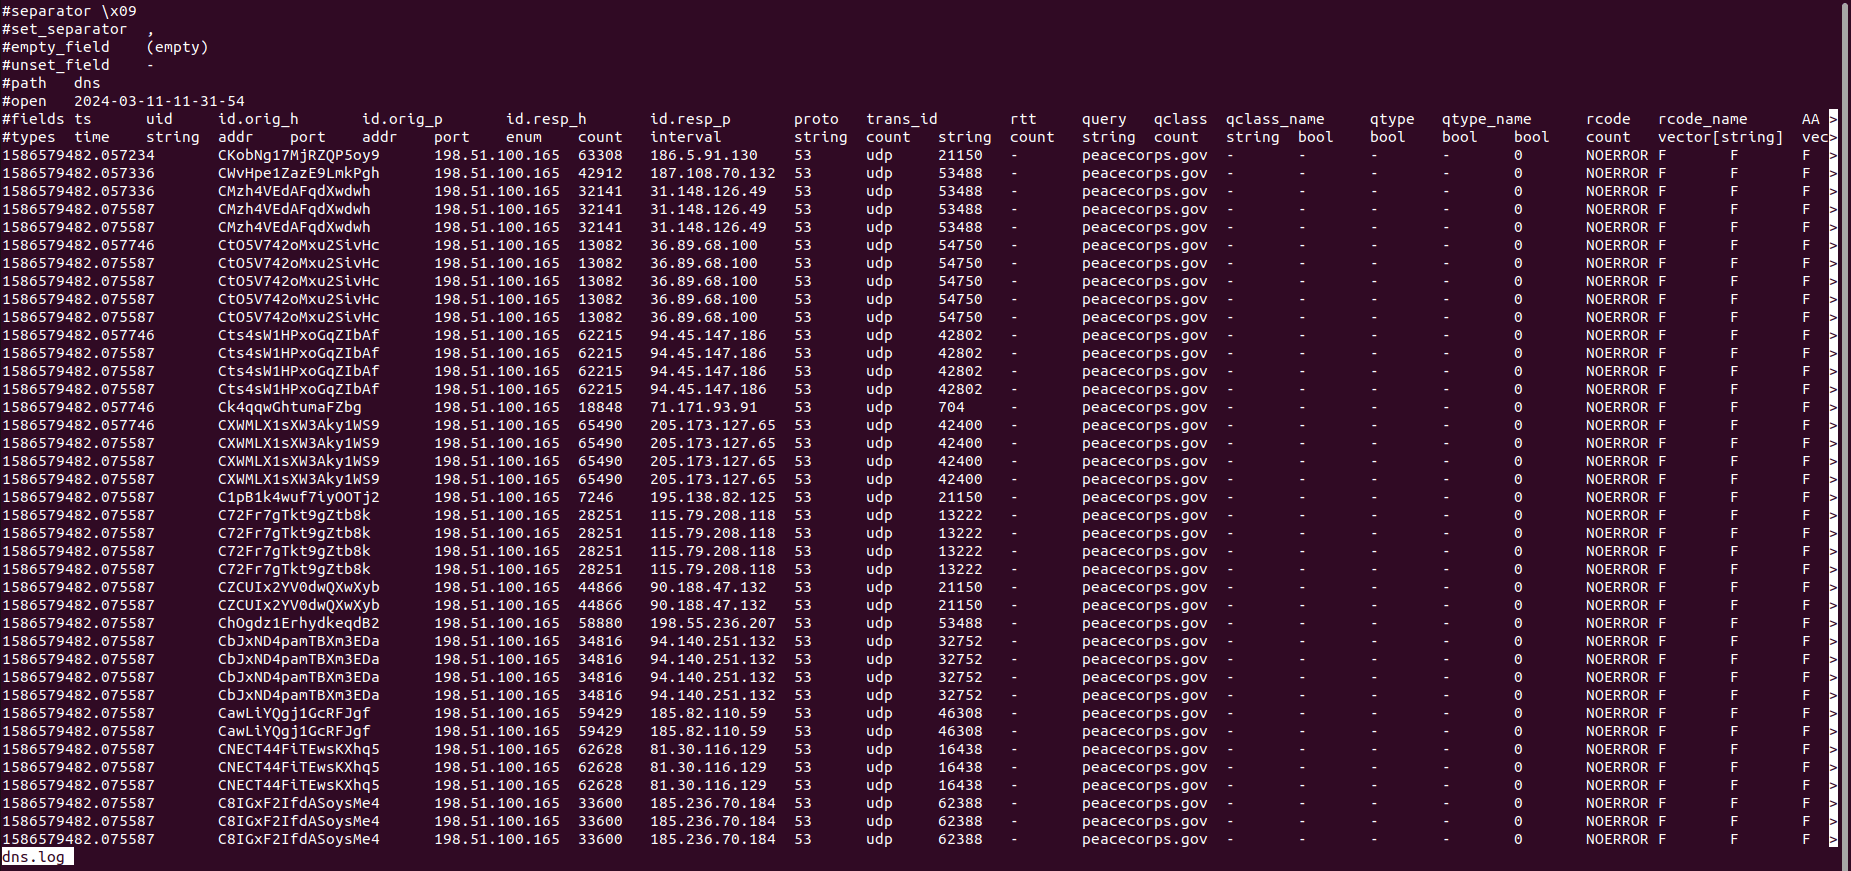
\includegraphics[width=1\linewidth]{images/pcap/pcap_3.png}
    \caption{show dns.log}
    \label{fig:enter-label}
\end{figure}

\begin{itemize}
    \item The execution of \texttt{cat dns.log | zeek-cut query | sort | uniq -c | sort -n}
 serves a critical function in aggregating and quantifying unique DNS queries. This pipeline first extracts the query field from the dns.log using zeek-cut, then sorts and counts unique instances, and finally orders them numerically.\\
    The output of the final command reveals the frequency of individual DNS queries, exemplified by 161 peacecorps.gov. This indicates that the domain peacecorps.gov was queried 161 times, highlighting it as a significant point of interest in the network traffic analyzed.
\end{itemize}


\begin{figure}[H]
    \centering
    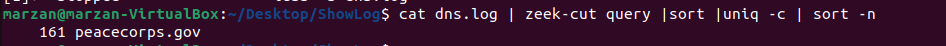
\includegraphics[width=1\linewidth]{images/pcap/pcap_5.png}
    \caption{zeek-cut for unique query}
    \label{fig:enter-label}
\end{figure}
